\documentclass[a4paper, 11pt]{article}

\title{\vspace{-3.0cm}Coursework 1: Report}
\author{
  Symbols, Patterns and Signals\\
  Dameli Ryspayeva\\
  Joshua Van Leeuwen
}

\date{}

\usepackage[margin=1in]{geometry}
\usepackage{graphicx}
\usepackage{amsmath}
\usepackage{subfig}
\begin{document}
\maketitle



\section*{\vspace{-0.35cm}Introduction}

\section*{\vspace{-0.35cm}Feature Selection}
Given the training set data we needed to identify which two features separate the classes of the data in order to know what attributes to use. To do this we visually inspected the data by plotting each pair of attribute values against each other. The results were:


\captionsetup[subfigure]{labelformat=empty}
\begin{figure}[h!]
    \centering
    \subfloat[Josh]{{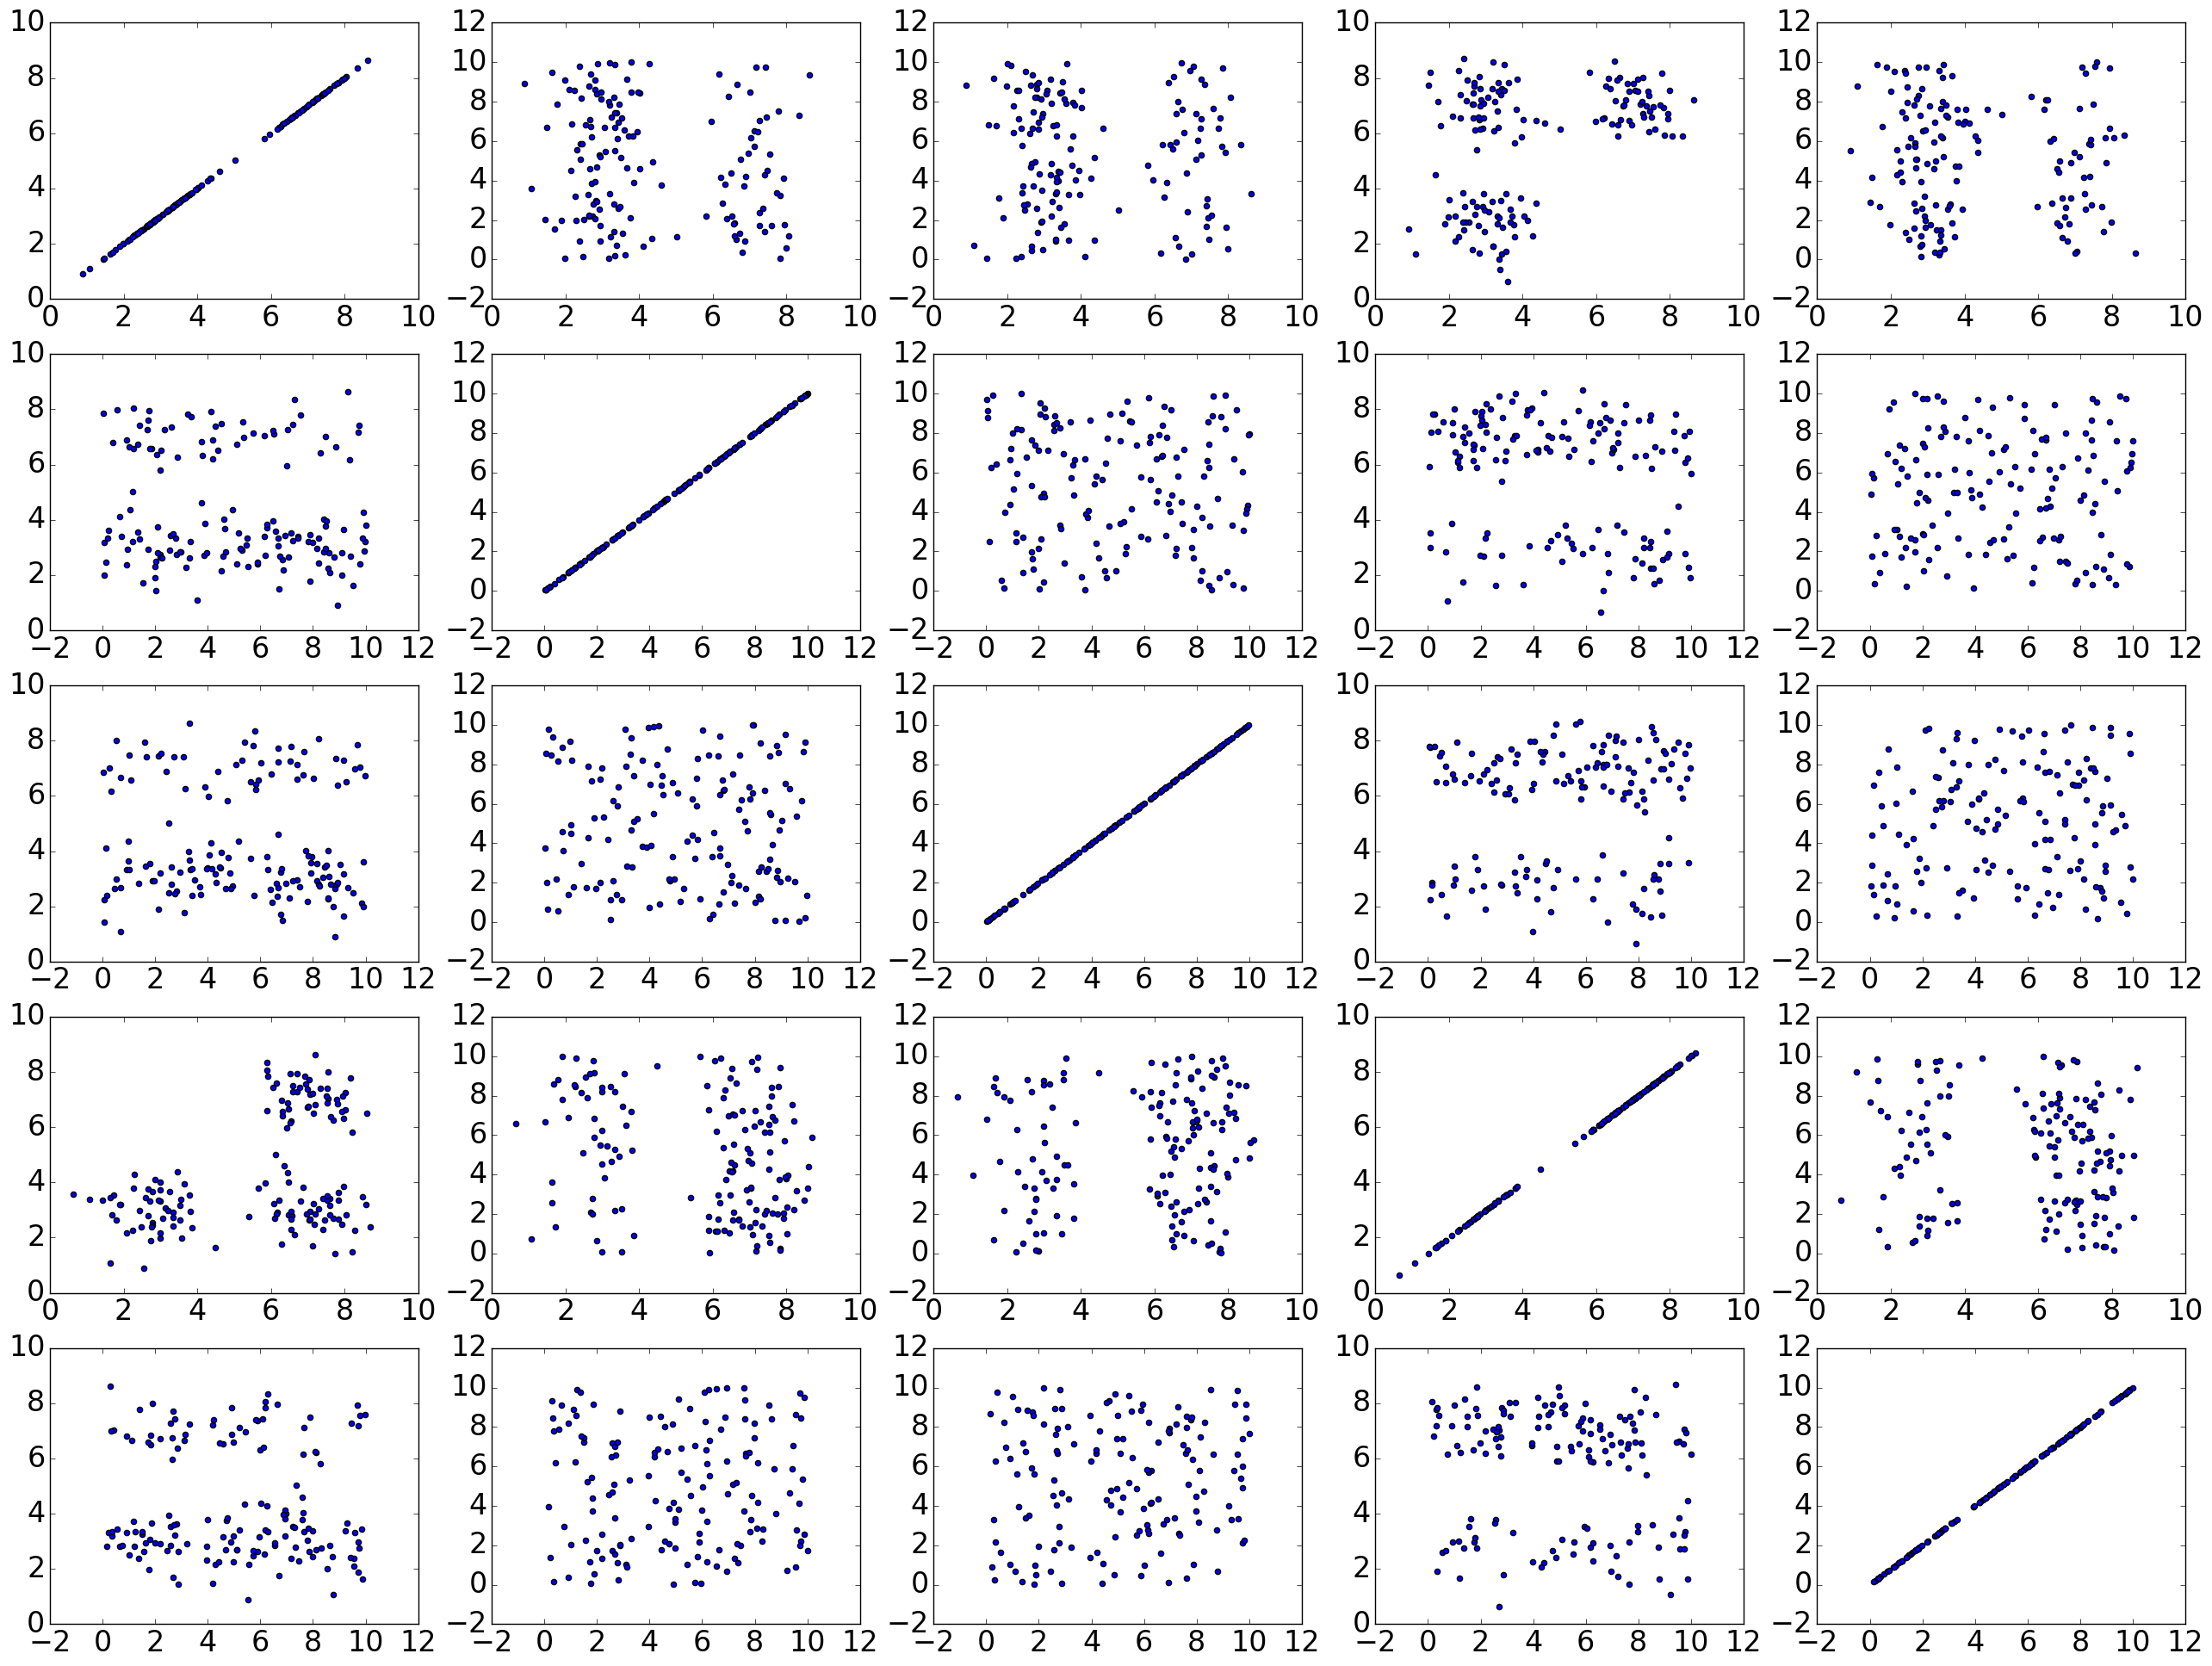
\includegraphics[width=7cm]{attributePlotJosh} }}%
    \qquad
    \subfloat[Dameli]{{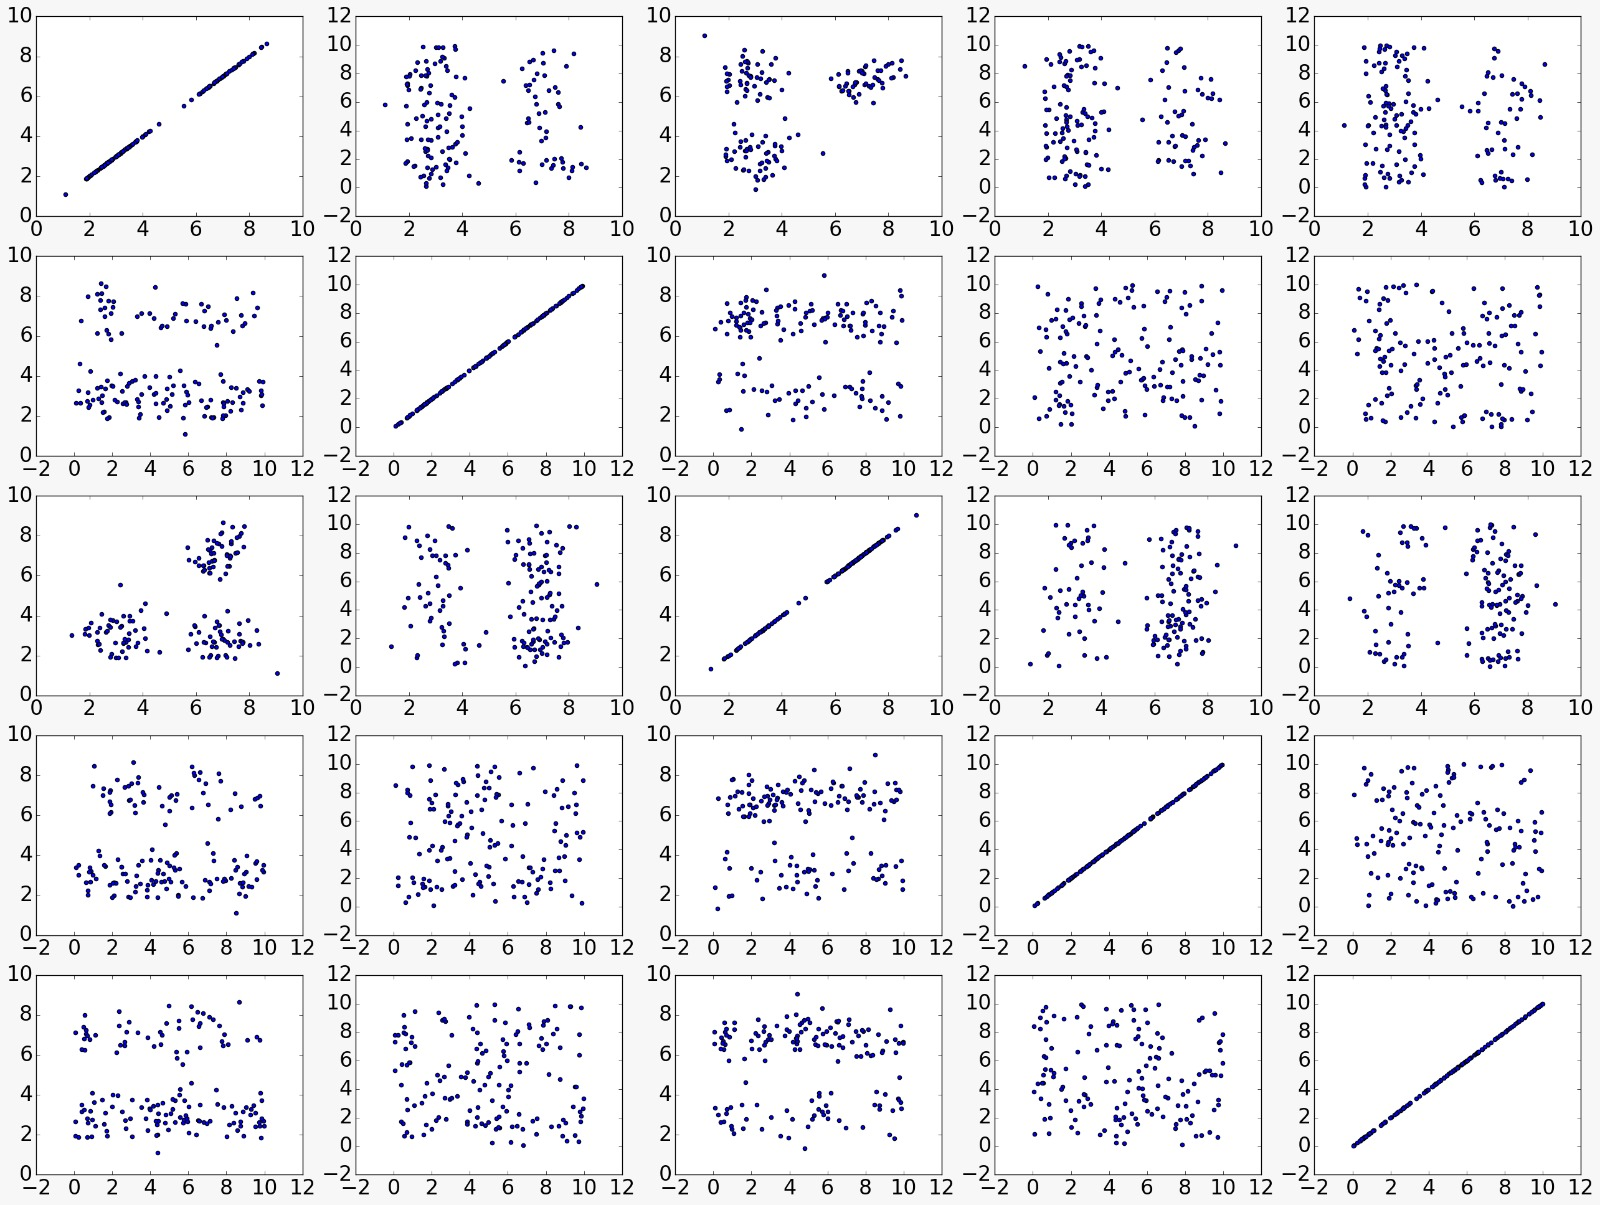
\includegraphics[width=7cm]{attributePlotDameli} }}%
    \caption{Attribute Plots}%
\end{figure}


Inspecting the graphs it is clear that in Figure 1, the attributes that separate the classes into clusters the most for the first set are the first and fourth attribute values whereas the first and fourth attribute values for the second set separate the data into clusters the most. This means that these attributes make up the features of their data sets.


\section*{\vspace{-0.35cm}Identifying the Classes}
Now we have identified that there are three classes displayed by the three clusters we then applied K-means to the data set to obtain the 3 clusters. By using K-means we were able to identify which data points belongs to which clustering. With this information we were able to visualise the different groupings using colour as shown by Figure 2.

\captionsetup[subfigure]{labelformat=empty}
\begin{figure}[h!]
    \centering
    \subfloat[Josh]{{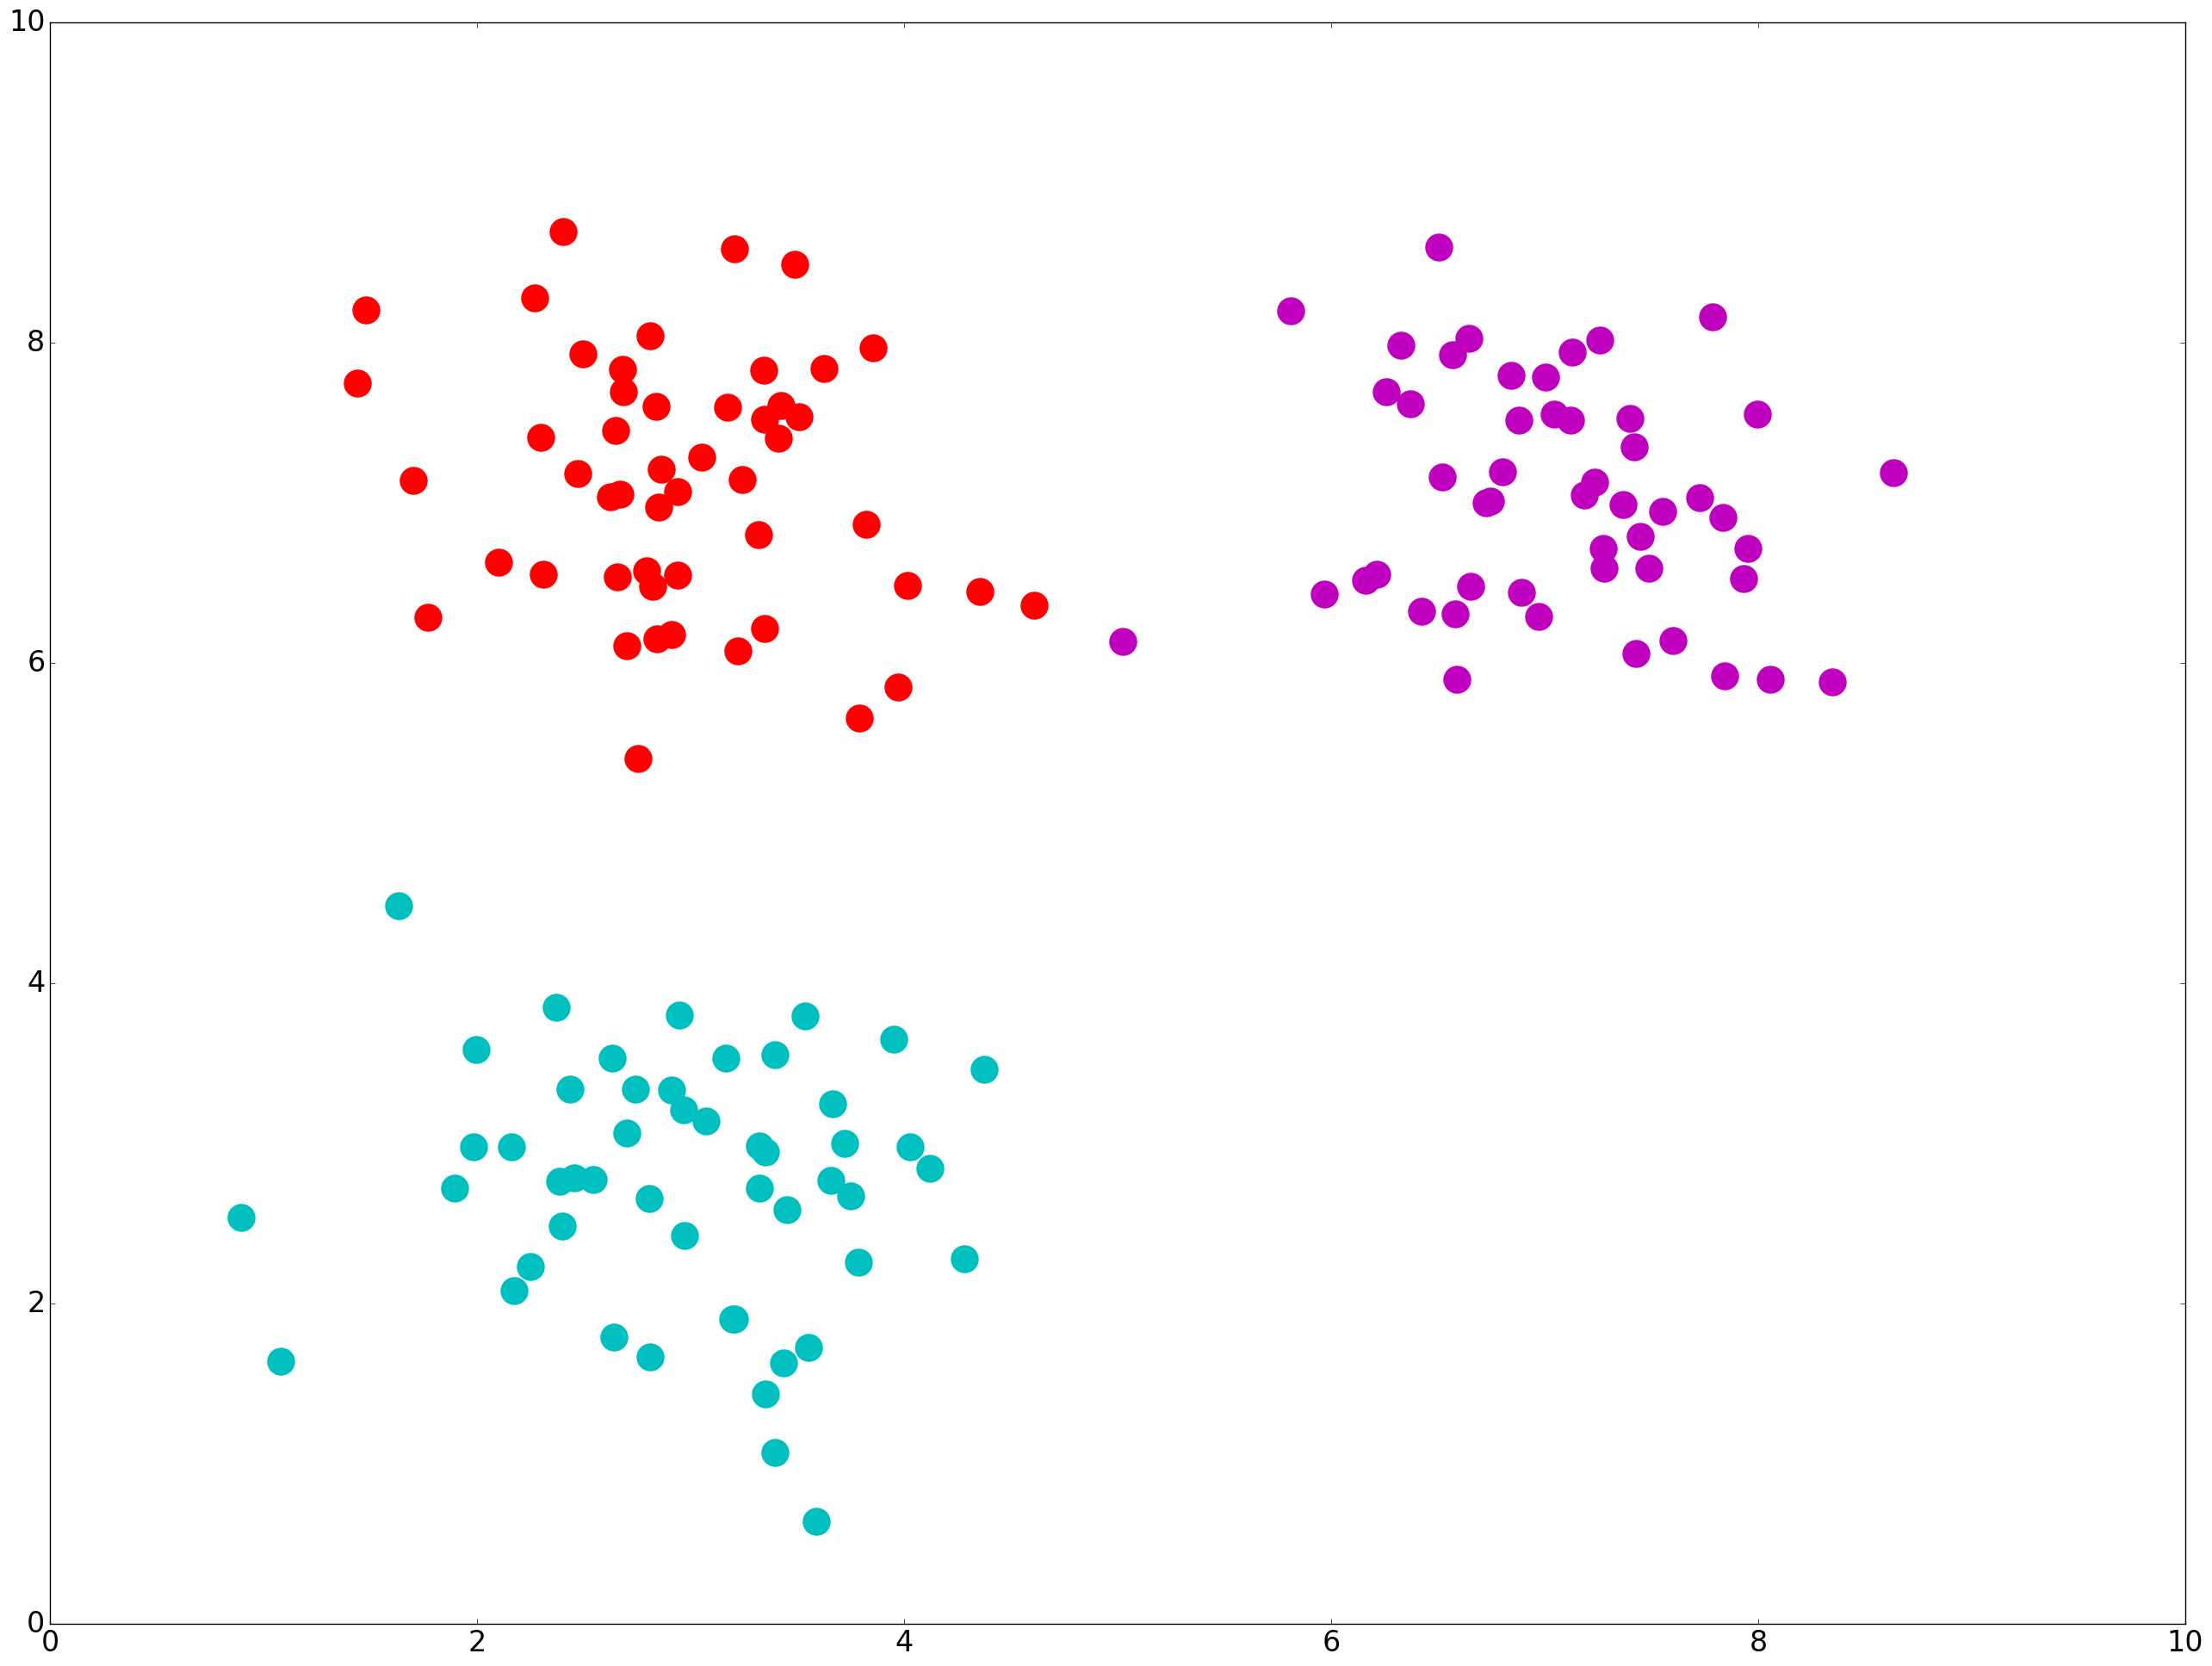
\includegraphics[width=7cm]{josh/joshORIGN} }}%
    \qquad
    \subfloat[Dameli]{{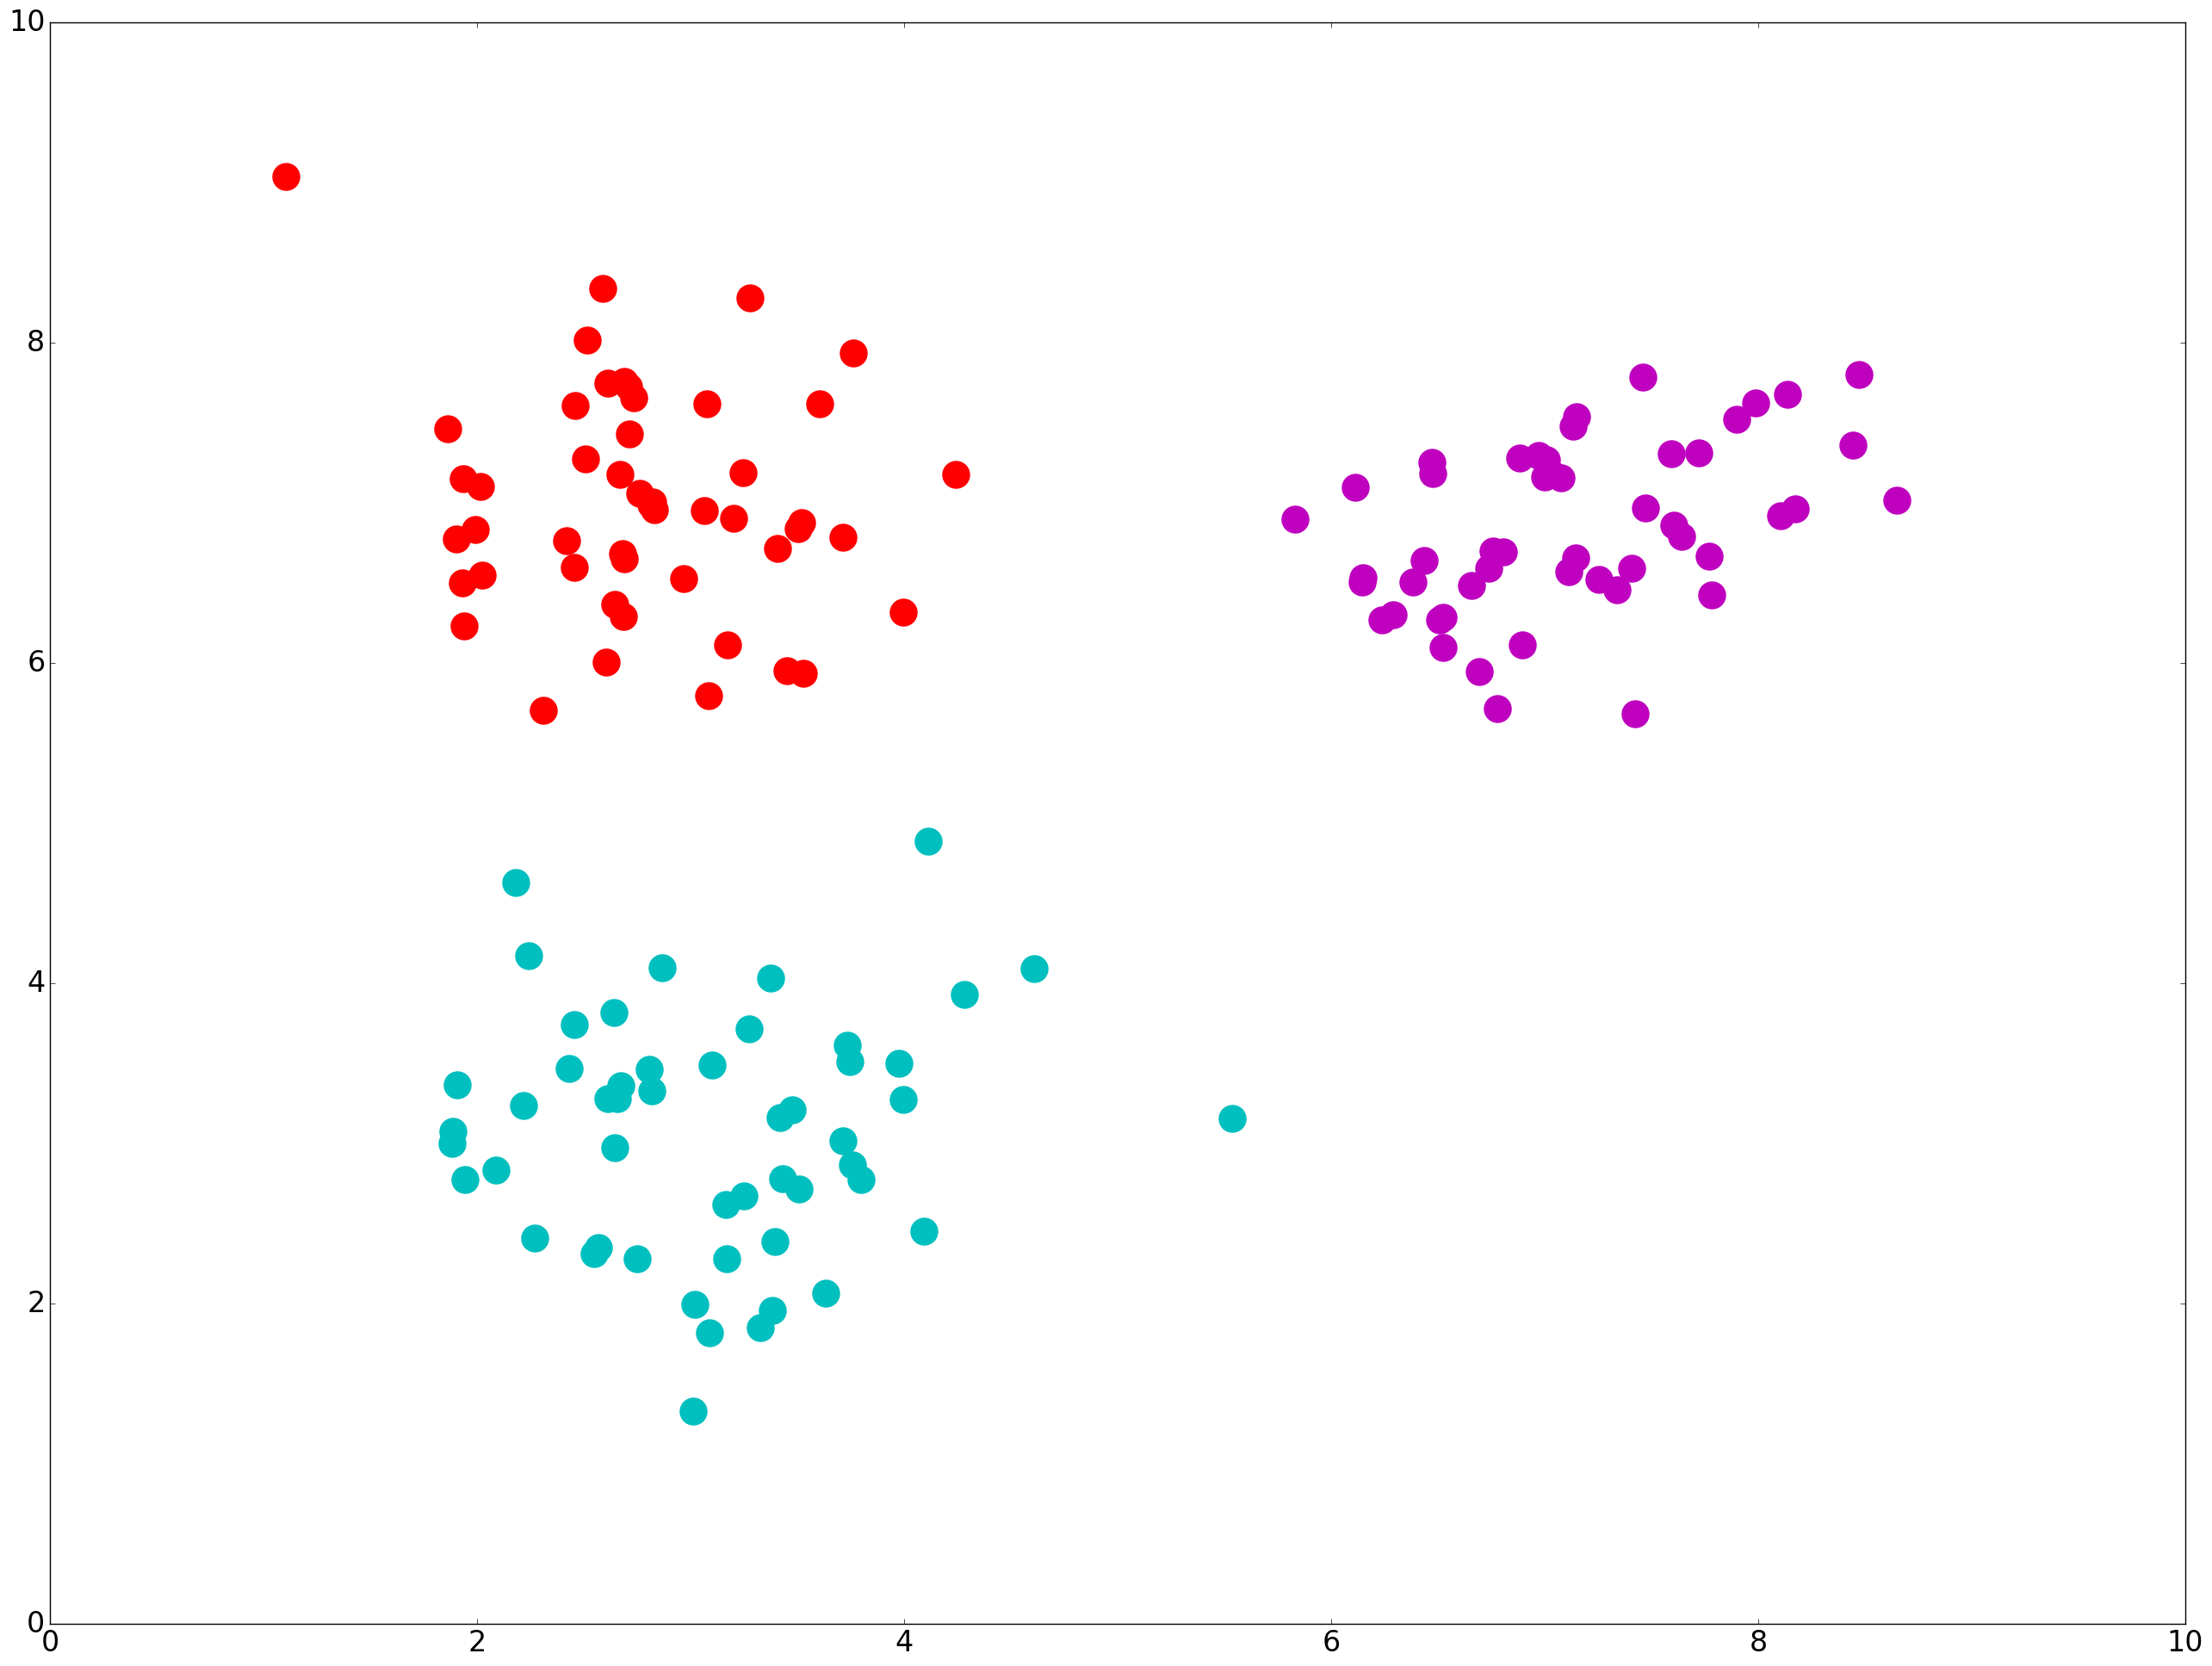
\includegraphics[width=7cm]{dameli/dameliORIGN} }}%
    \caption{Nearest-centroid classification}%
\end{figure}

The result of visualising K-means and assigning the points to a class is what we expected as it has matched what we thought the clustering should be. K-means is a centroid-based clustering algorithm which partitions features into several sets of data that we refer to, as clusters, by minimising the within-cluster sum of squares. Mathematically, this is denoted as: 

\begin{equation*}
  \boldsymbol{\operatorname*{arg\,min}_S} \sum_{i=1}^{k}\sum_{\boldsymbol{x} \epsilon S_i}  \boldsymbol{\parallel x - \mu_{i} \parallel^{2}}
\end{equation*}

where
S is a set of clusters, x is the set of observations and k is the number of clusters. \cite{wikiKMeans}\\

According to the number of clusters, n, the algorithm randomly initialises n points that are called centroids. Given that K-means is an iterative algorithm, it iteratively continues doing two steps: assigning a point to a cluster and moving centroids closer to the centre of this cluster. In our case, it will go through each point of the features set and will assign them to one of the cluster groups depending on which cluster is closer to that point. After that, it will recalculate the average of all points within a cluster according to the formula below and will assign the centroid to the current centre of the cluster. The two steps are repeated until the centroid value no longer changes.

\begin{equation*}
  \boldsymbol{v}_i = \boldsymbol{(1/c}_i) \boldsymbol{\sum_{j=1}^{c_i} x_i}_{\cite{K-Means}}
\end{equation*}

Given that the final result depends on the very first step when centroids are placed randomly, the algorithm should be repeated a lot of times no matter whether optimal or non-optimal clustering needs to be achieved. To identify the best result, cluster distortion, the sum of the squared differences between each features’ point and its corresponding centre of the cluster it belongs to, needs to be examined. The clustering with the lowest distortion will be an indication of the best clustering. \cite{BigData}


However, the clustering with the lowest distortion will not signify the worst one. For this purpose the algorithm needs to be modified as it optimises the centroids by moving them closer to the cluster centres. So, to achieve the non-optimal clustering, centroids should be placed randomly and the new cluster centre should never be recalculated. 

The differences between non-optimal and best clustering can be seen by comparing the plots below:

\section*{\vspace{-0.35cm}Nearest-centroid Classification}
When classifying new data points into our set one can use the nearest-centroid classification algorithm to fit them into the correct class. We have done this with our test data set and have visualised it by adding them to the plots, shown in Figure 3.

\captionsetup[subfigure]{labelformat=empty}
\begin{figure}[h!]
    \centering
    \subfloat[Josh]{{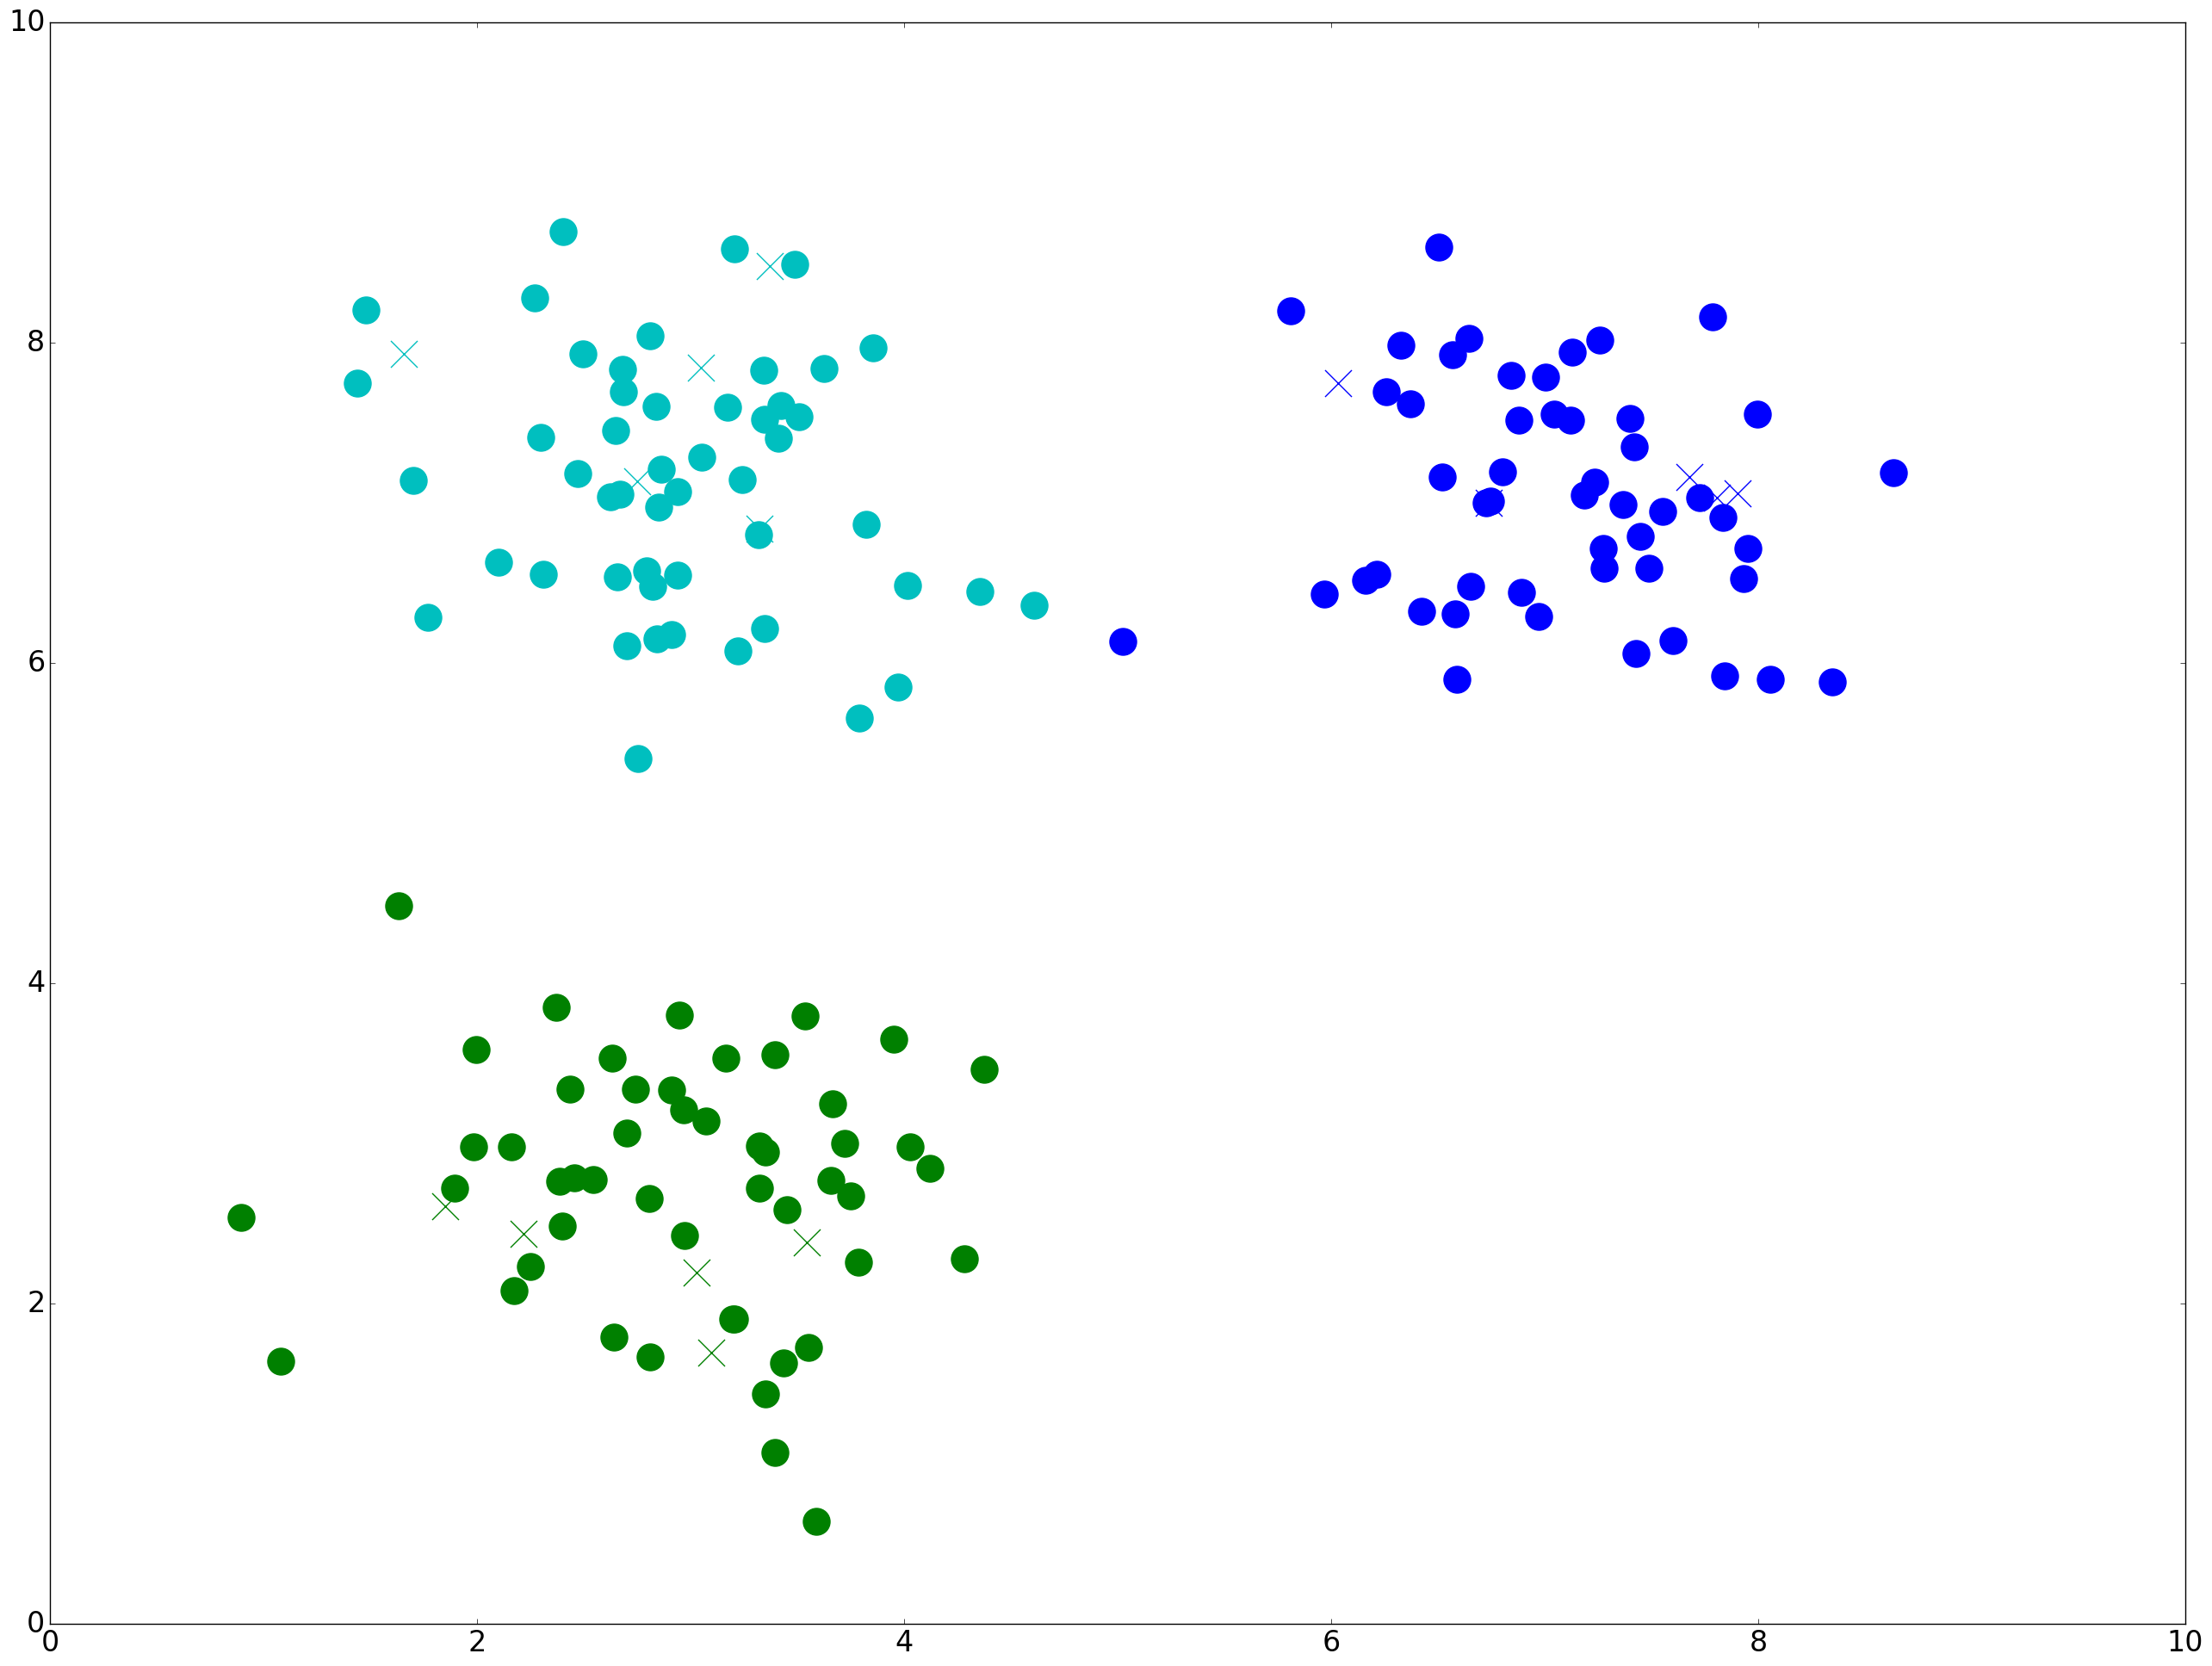
\includegraphics[width=7cm]{josh/joshTEST.png} }}%
    \qquad
    \subfloat[Dameli]{{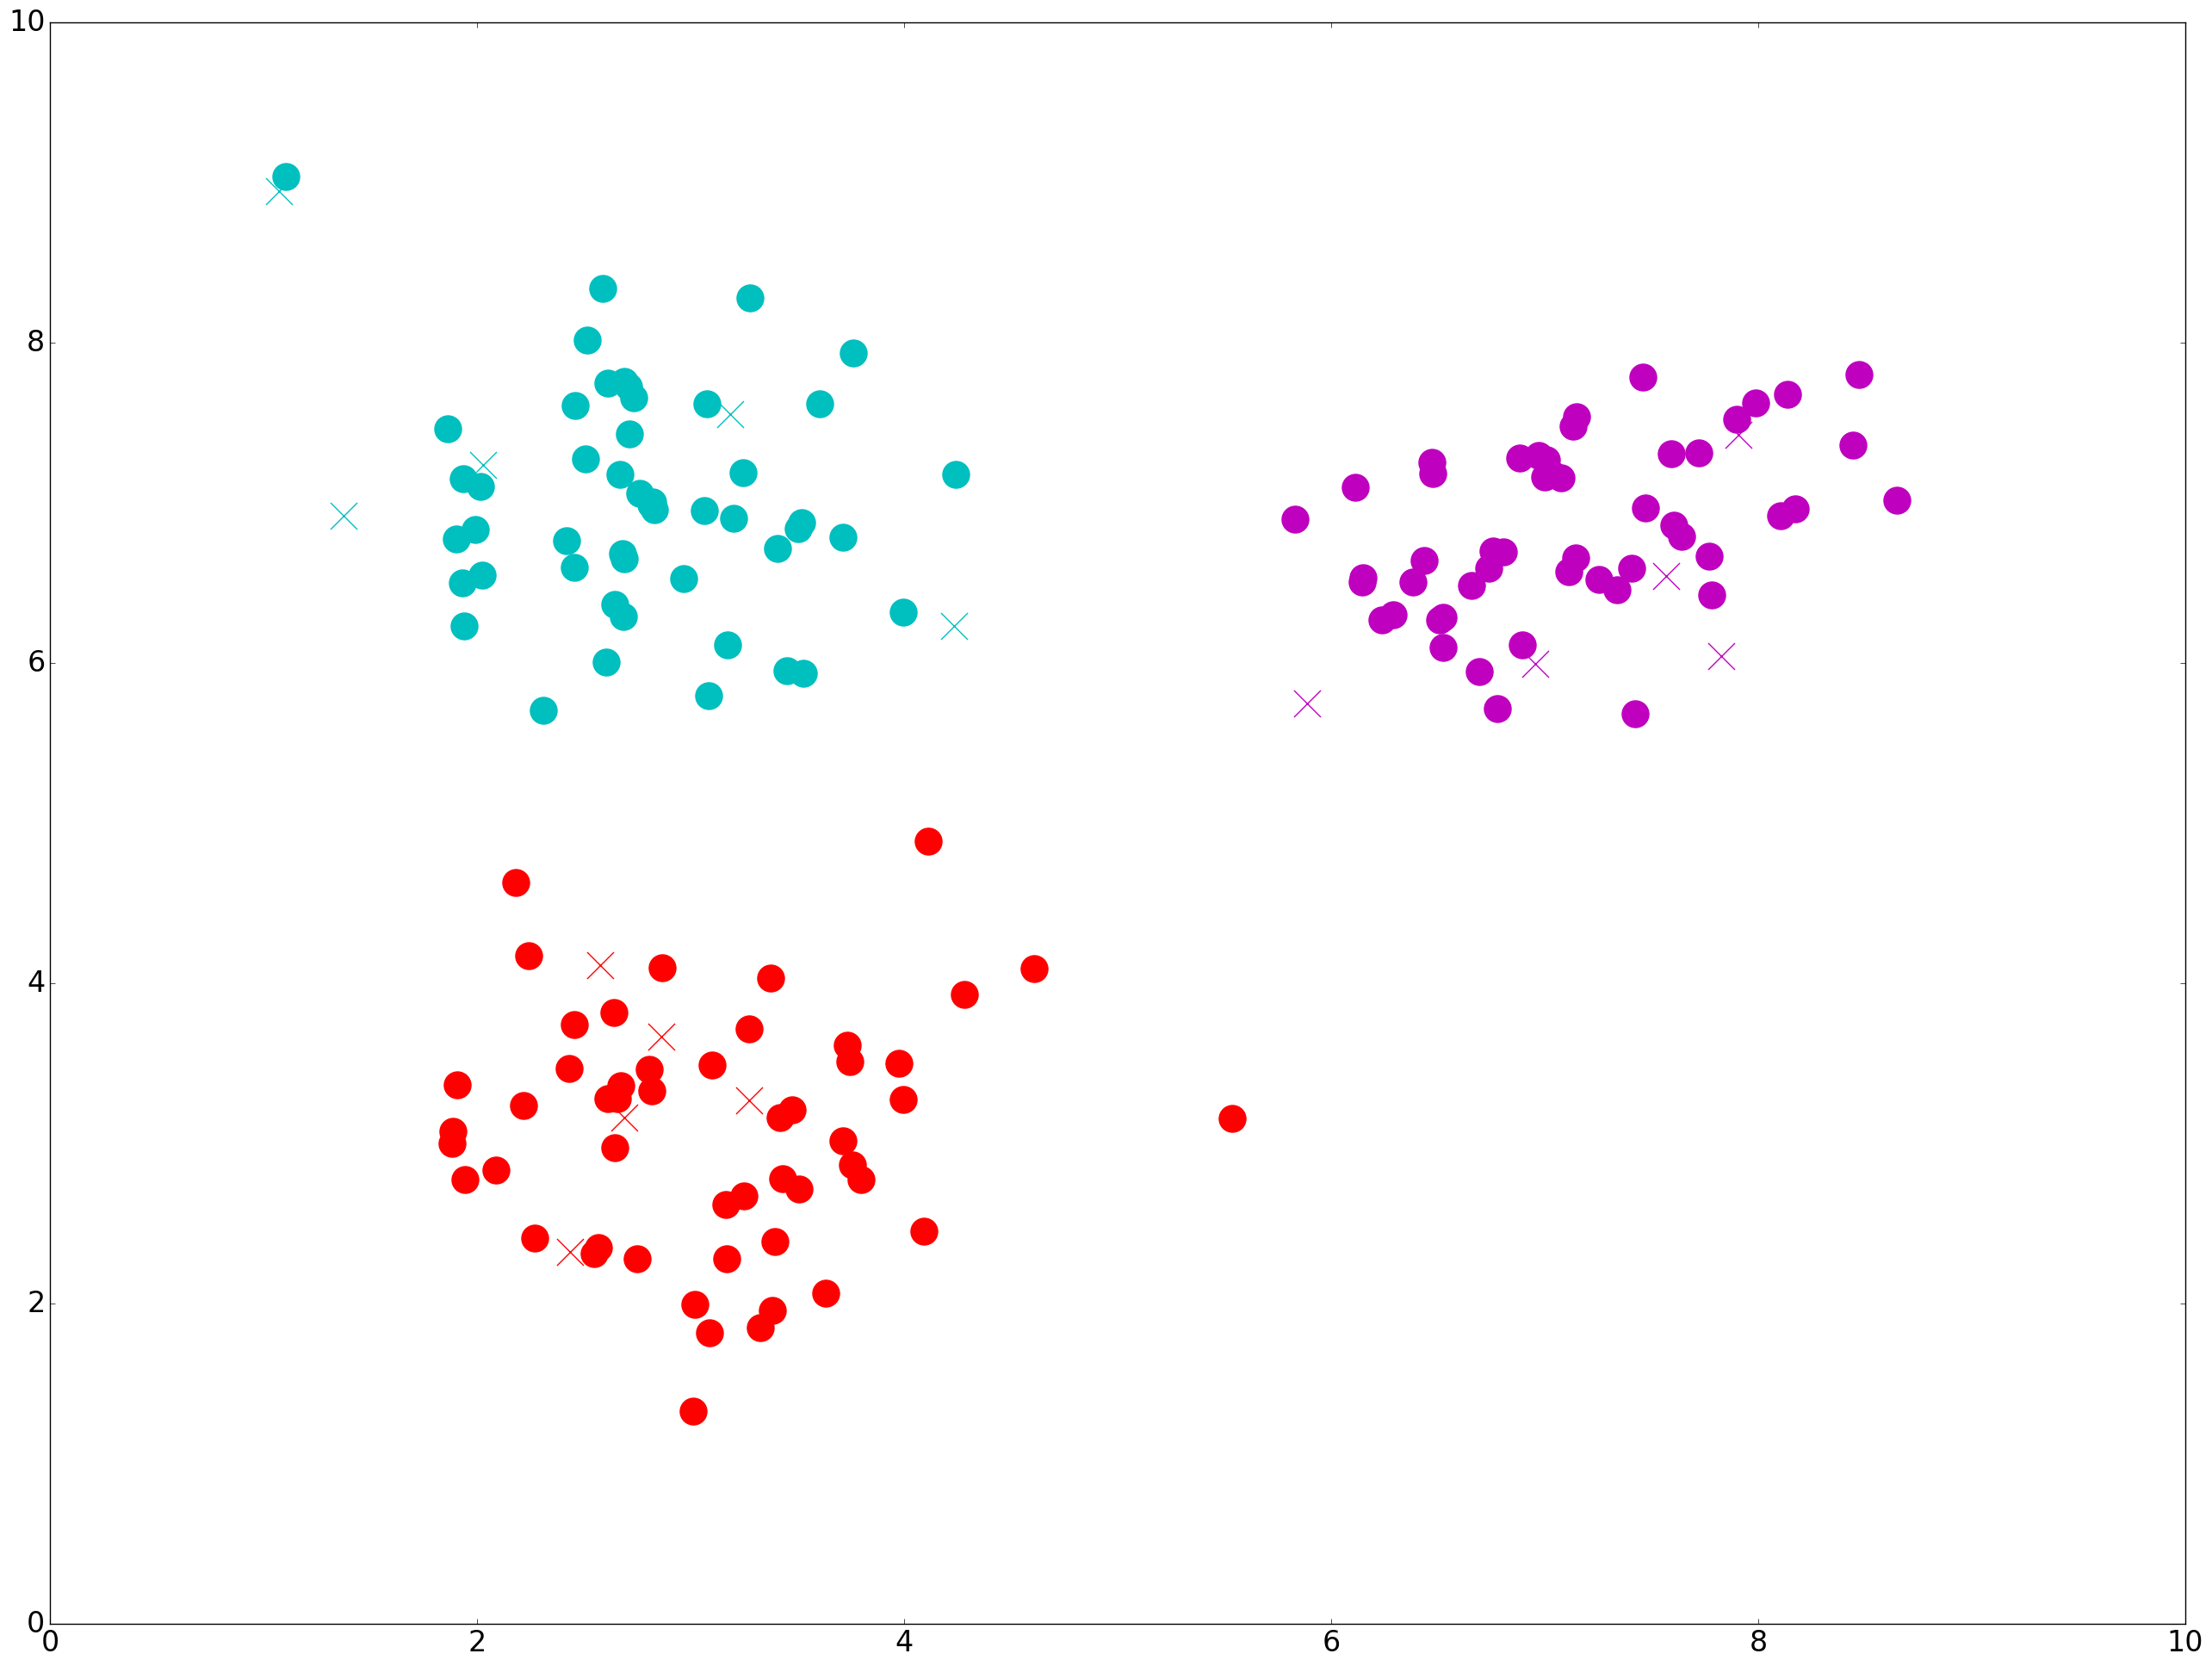
\includegraphics[width=7cm]{dameli/dameliNEARNEiGH.png} }}%
    \caption{Nearest-centroid classification}%
\end{figure}


In order to achieve this we obtained the centroids of each class via the K-means algorithm stated before. We can then use the attribute values from the test set and obtain the feature values that we had chosen previously. With each of these 2-D points, we can treat them as vectors and use euclidean distance to determine which centroid is closest for every point in the test data. The closest centroid to a point will determine its class and thus be added to it. Figure 3 shows how the new points, denoted by an X, have been added to the classes that we would expect, given which cluster contains that point.

Using the centroids obtained by K-means we can also visualise the decision boundaries shown in Figure 4, using a Voronoi diagram. The Voronoi decision boundaries are calculated again, using the euclidean distances with the centroid points.

\captionsetup[subfigure]{labelformat=empty}
\begin{figure}[h!]
    \centering
    \subfloat[Josh]{{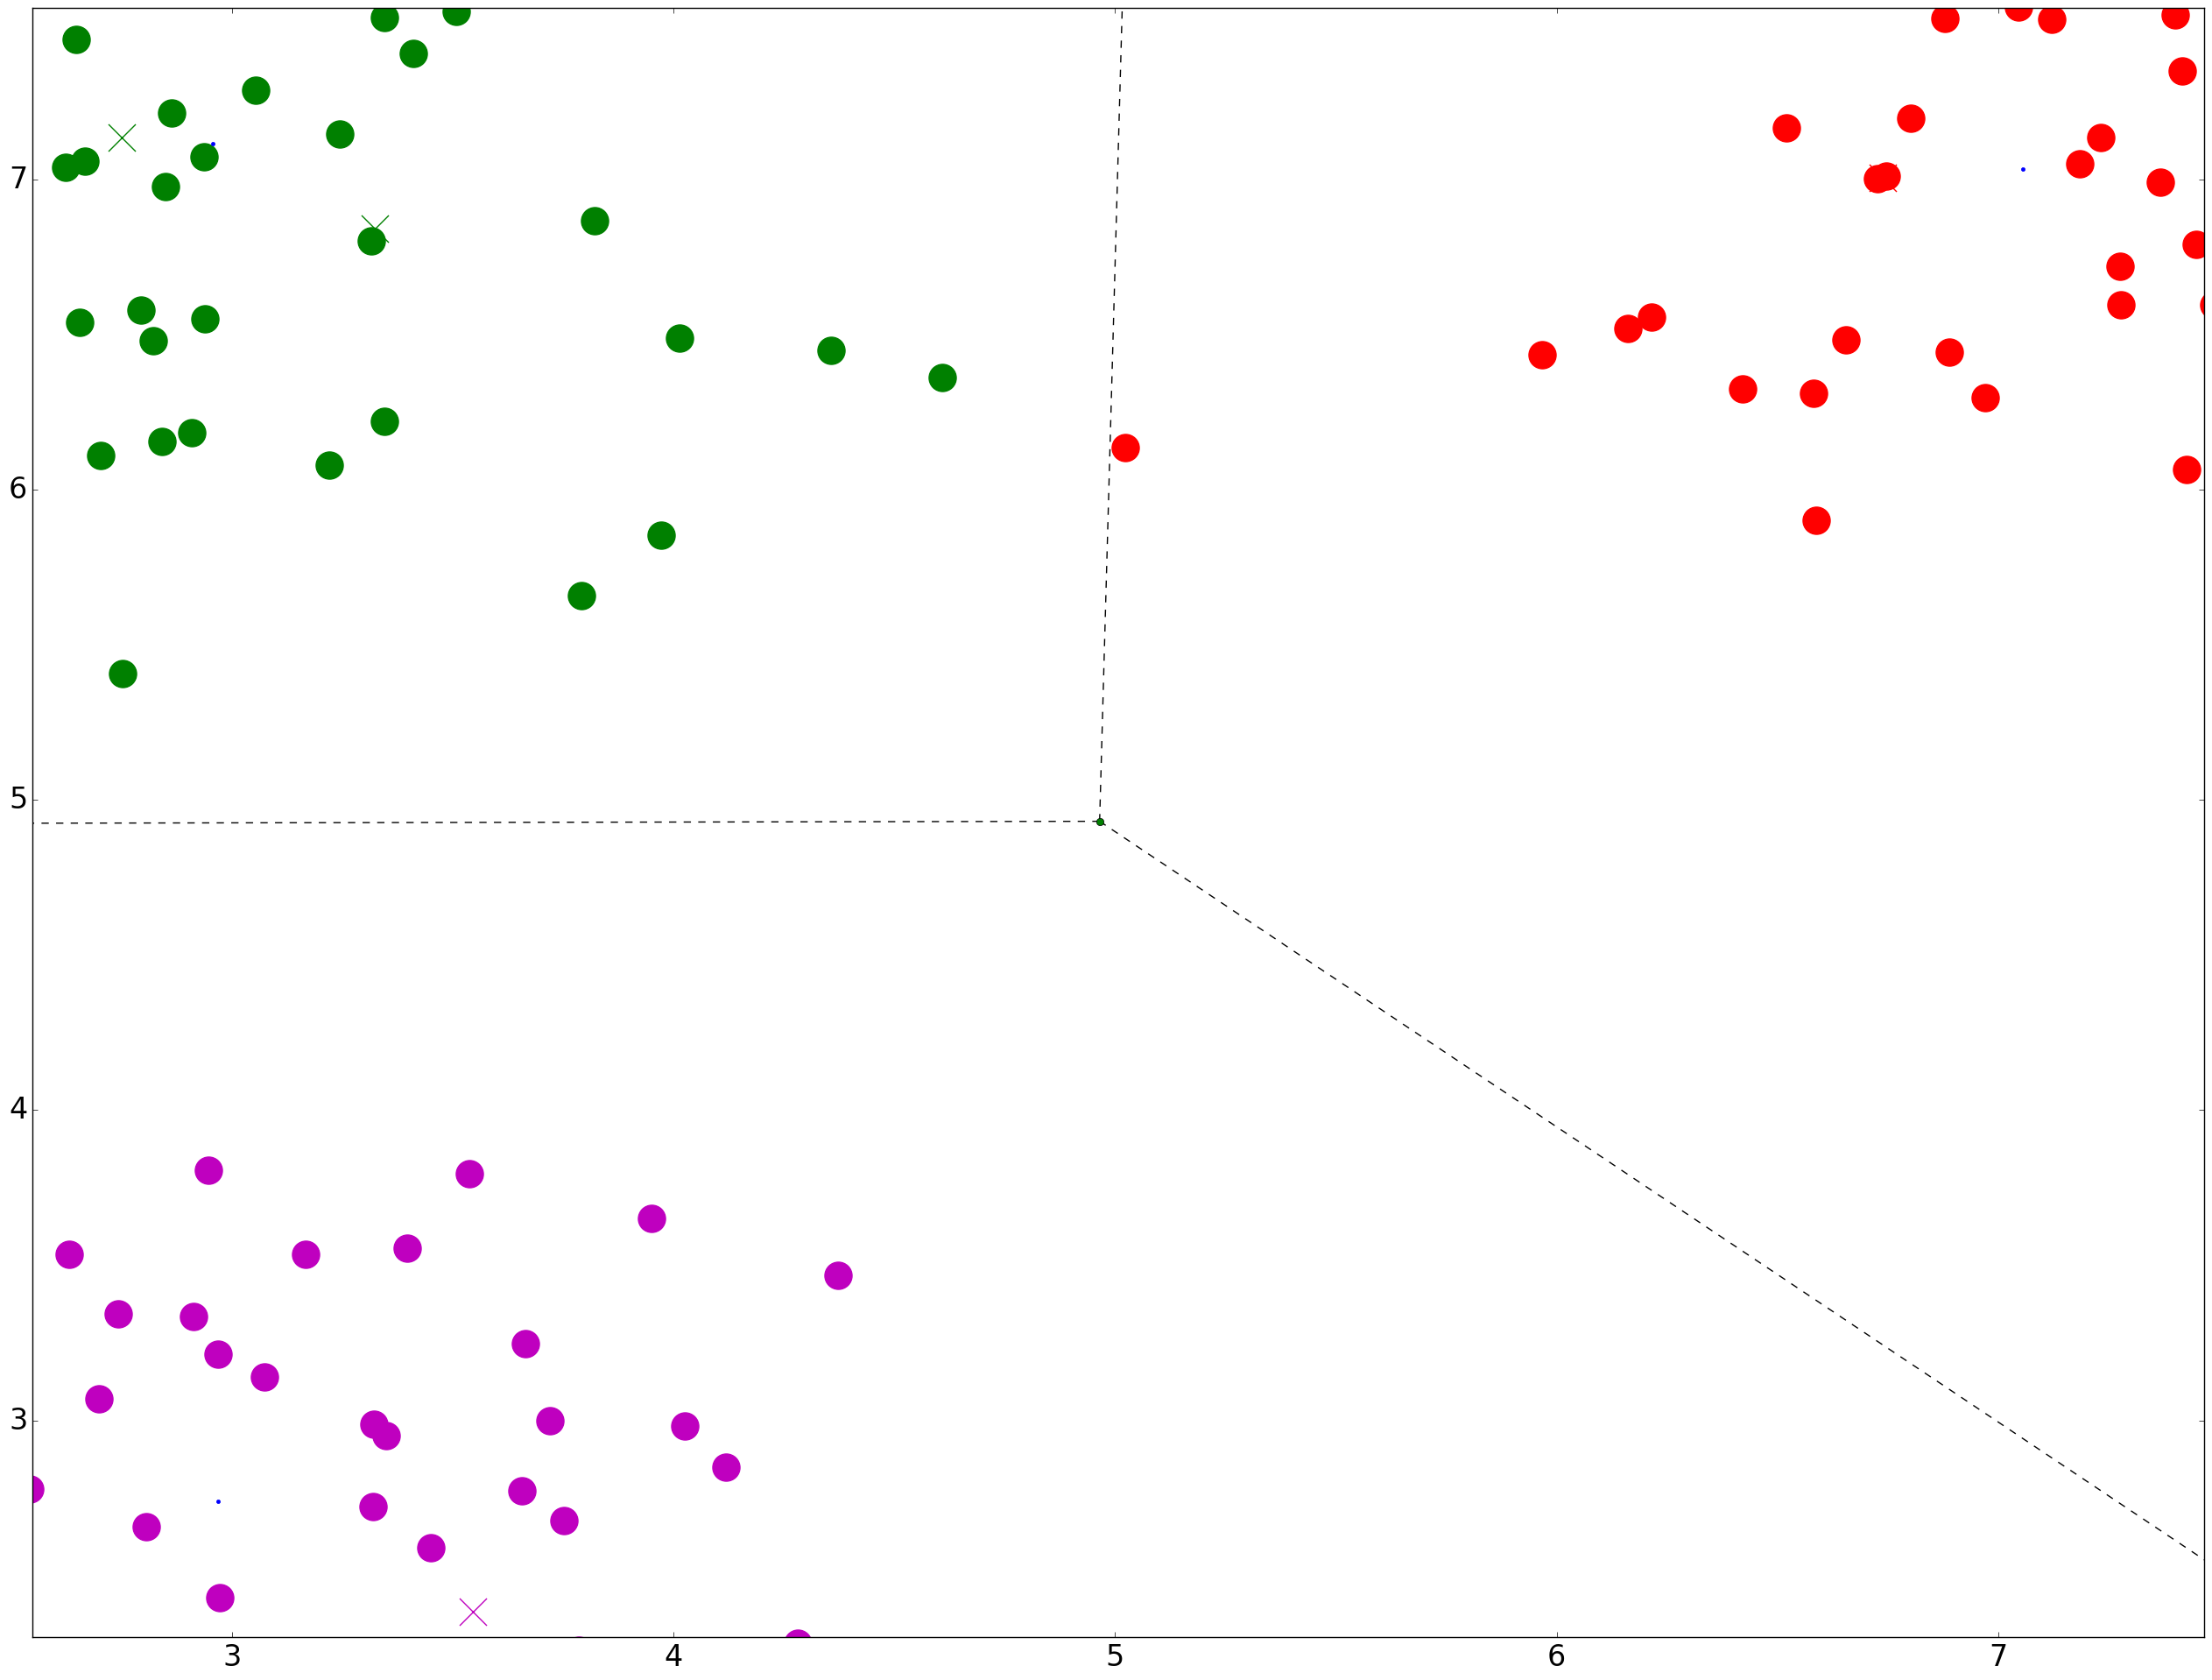
\includegraphics[width=7cm]{josh/joshVORON.png} }}%
    \qquad
    \subfloat[Dameli]{{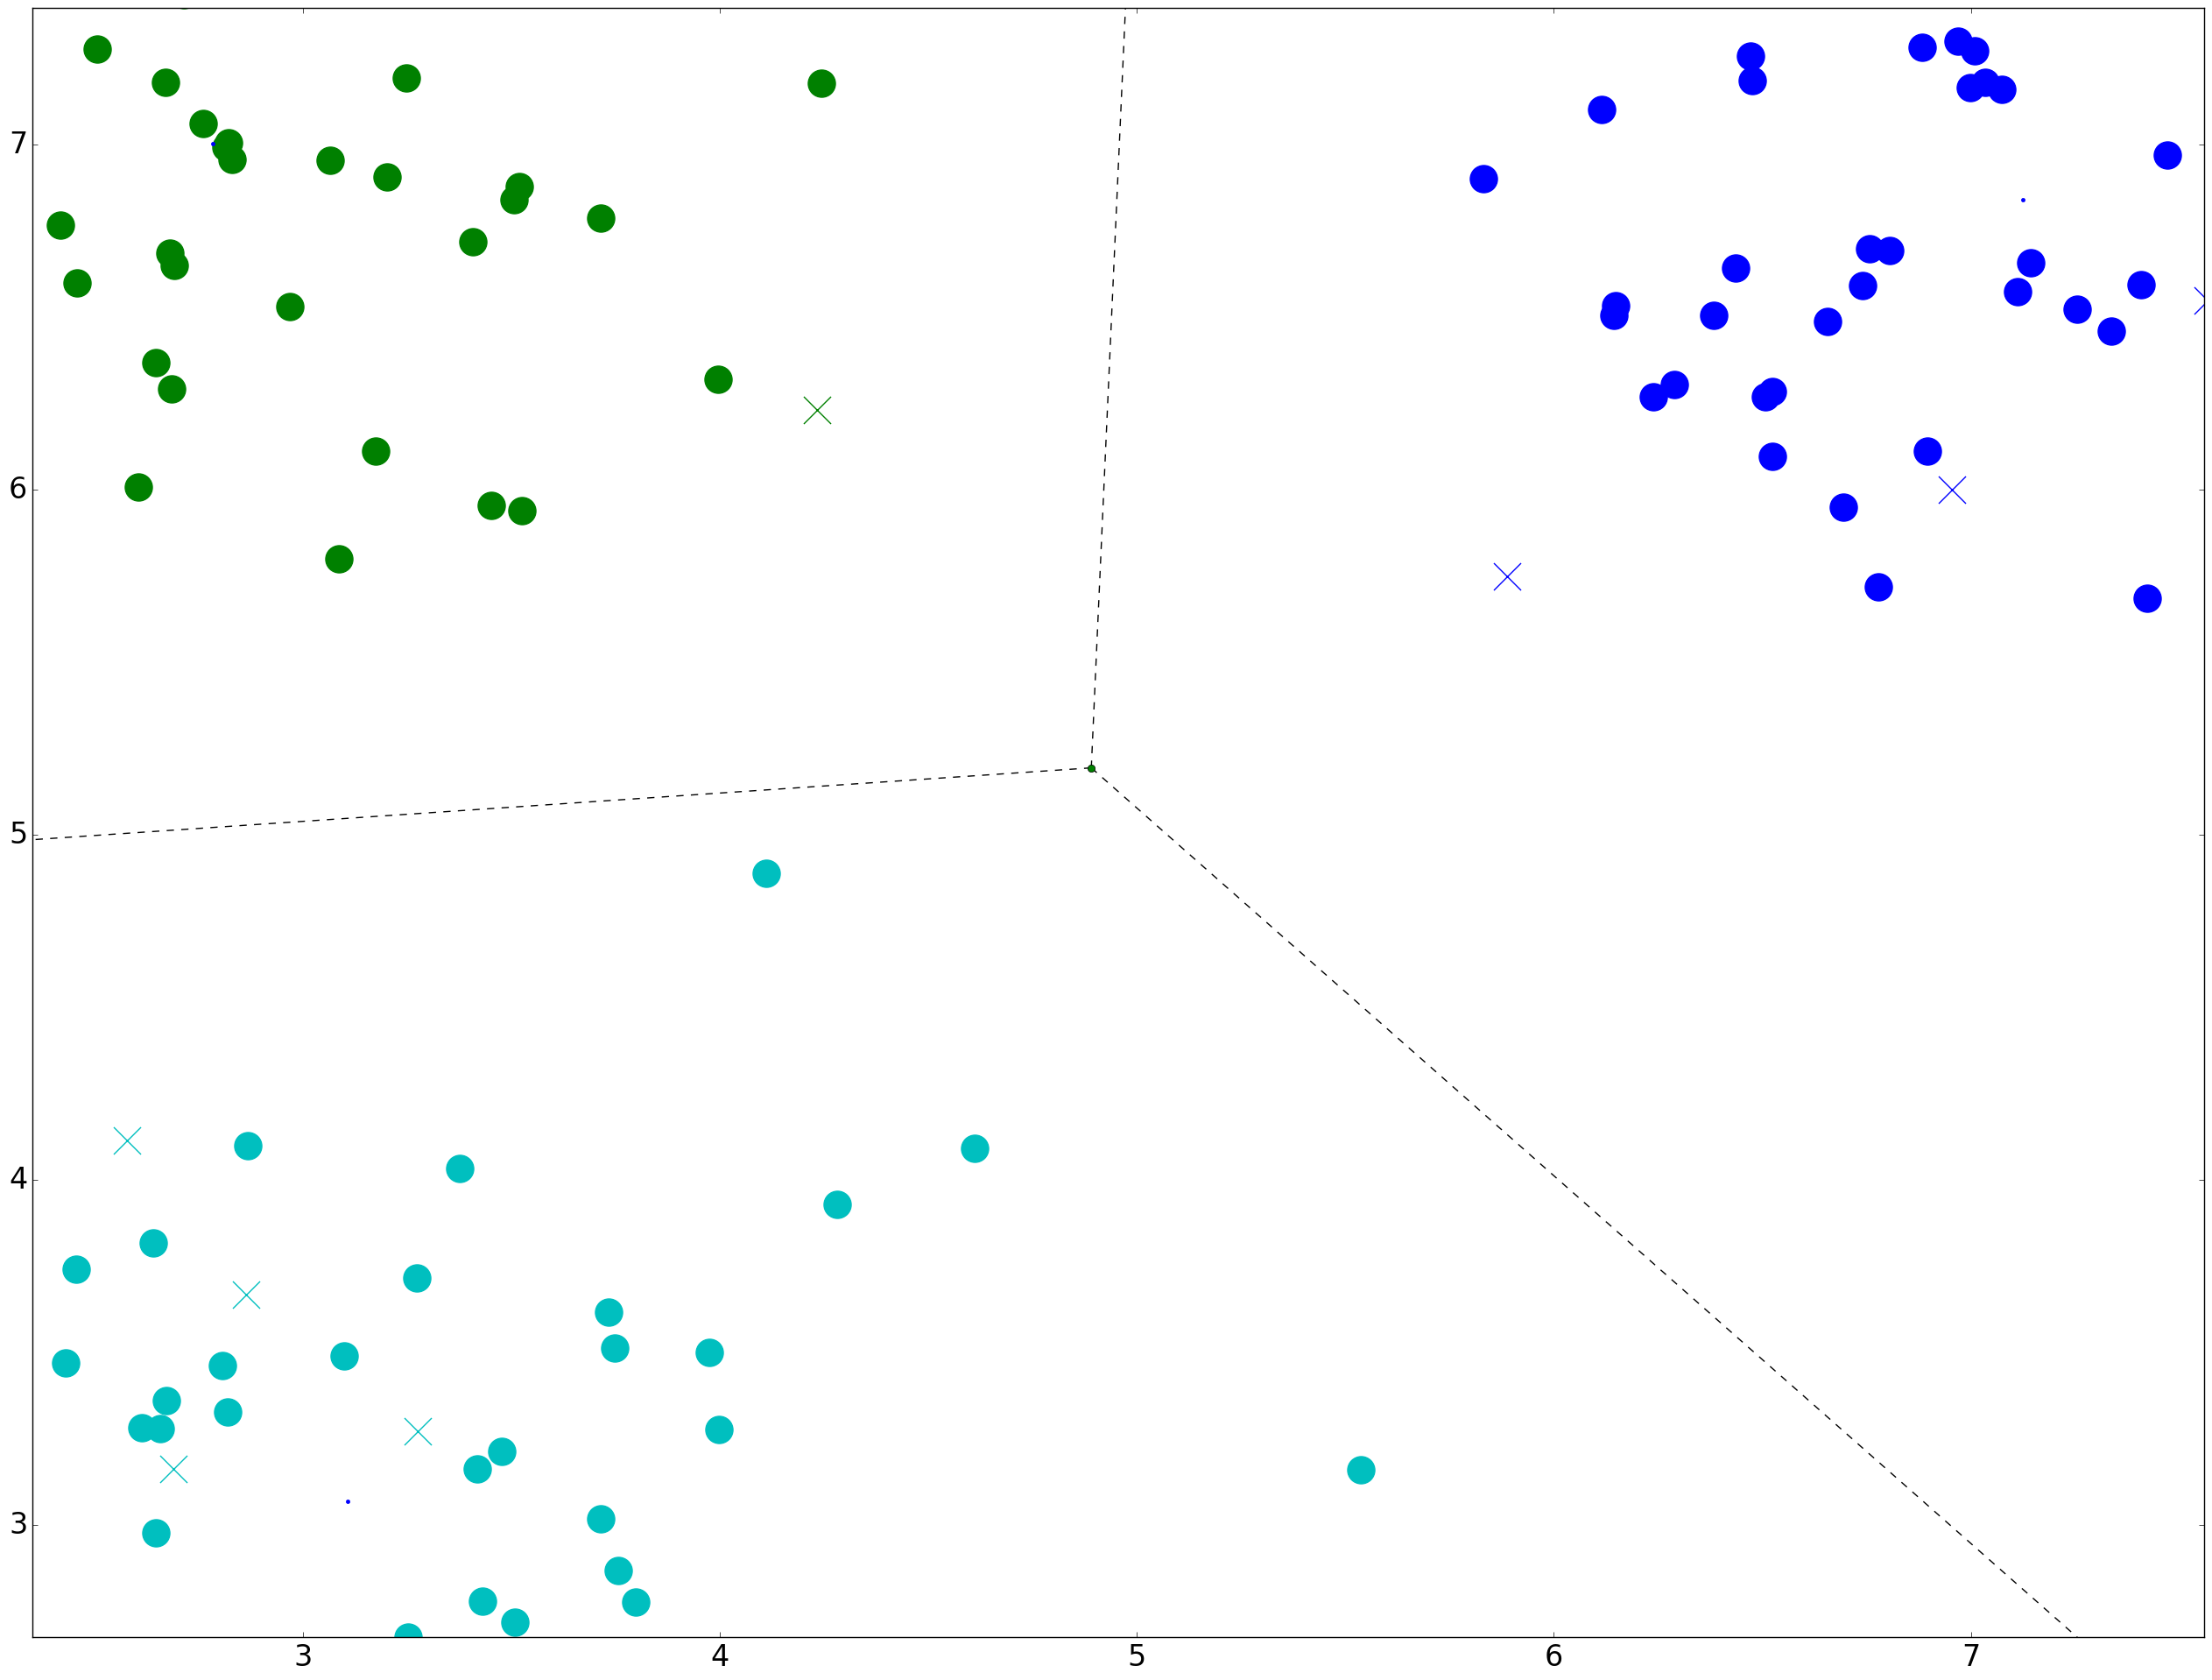
\includegraphics[width=7cm]{dameli/dameliVORON.png} }}%
    \caption{Decision boundaries with Voronoi diagram}%
\end{figure}


\section*{\vspace{-0.35cm}Maximum-likelihood Classification}

\section*{\vspace{-0.35cm}Discussion of Results}

\begin{thebibliography}{9}
    \bibitem{wikiKMeans}
     Wikipedia. 2017. k-means clustering - Wikipedia.
     \\\texttt{https://en.wikipedia.org/wiki/K-means\_clustering}
     
    \bibitem{K-Means}
     Big Data Made Simple - One source. Many perspectives.. 2017. Possibly the simplest way to explain K-Means algorithm.
     \\\texttt{http://bigdata-madesimple.com/possibly-the-simplest-way-to-explain-k-means-algorithm/.}

    \bibitem{BigData}
     k-means clustering algorithm - Data Clustering Algorithms. 2017. k-means clustering algorithm - Data Clustering Algorithms. 
     \\\texttt{https://sites.google.com/site/dataclusteringalgorithms/k-means-clustering-algorithm}

\end{thebibliography}

\end{document}
